\documentclass[twocolumn,superscriptaddress,prl,amsmath,amssymb]{revtex4-2}

\usepackage{graphicx}
\usepackage{dcolumn}
\usepackage{bm}
\usepackage{hyperref}
\usepackage{amsmath}
\usepackage{amssymb}
\usepackage{xcolor}

\begin{document}

\title{Holographic Derivation of the IAM Activation Function:\\From Horizon Thermodynamics to Dual-Sector Cosmology}

\author{Heath W. Mahaffey}
\email{hmahaffeyges@gmail.com}
\affiliation{Independent Researcher, Entiat, WA 98822, USA}

\date{\today}

\begin{abstract}
The Informational Actualization Model (IAM) introduces a structure-dependent activation function $\mathcal{E}(a) = \exp(1 - 1/a)$ into the Friedmann equation, resolving the Hubble tension at $5.6\sigma$ over $\Lambda$CDM. While this function was introduced phenomenologically in the main manuscript, we derive here its functional form from first principles using horizon thermodynamics. The derivation proceeds from three established results: (i) the Bekenstein-Hawking entropy-area relation, (ii) the Gibbons-Hawking horizon temperature, and (iii) Landauer's principle applied to irreversible information production from gravitational decoherence. The key result is that cosmic expansion responds to information \textit{surface density} on the horizon---the ratio of the structure formation rate to the horizon area. During matter domination, this ratio scales as $1/a^2$, whose integral gives $-1/a + C$. Exponentiation with appropriate normalization recovers $\mathcal{E}(a) = \exp(1 - 1/a)$ exactly. Numerical verification using Press-Schechter halo collapse rates with Gibbons-Hawking temperature corrections produces $\exp(\alpha - \beta/a)$ with $\alpha \approx 0.95$--$1.04$ and $\beta \approx 1.05$--$1.18$ depending on the nonlinear source model, matching the phenomenological form to within $5$--$15\%$ across a range of physically motivated decoherence rates (Pearson $r > 0.98$). The photon exemption ($\Sigma = 1$) and growth suppression ($\mu < 1$) emerge automatically: photons do not undergo gravitational decoherence and therefore contribute zero to the informational entropy term. This elevates IAM from a phenomenological fit to a physically motivated cosmological framework grounded in horizon thermodynamics.
\end{abstract}

\maketitle

%% ============================================================
%% SECTION 1: INTRODUCTION
%% ============================================================
\section{Introduction}

The Informational Actualization Model (IAM) was introduced in the companion manuscript~\cite{Mahaffey2026main} as a phenomenological resolution to the Hubble tension. By adding a structure-dependent term $\beta\mathcal{E}(a)$ to the Friedmann equation, with activation function $\mathcal{E}(a) = \exp(1 - 1/a)$, the model produces distinct expansion rates for matter-based and photon-based observables. Comprehensive validation against Planck, SH0ES, Pantheon+, and DESI data yields $\Delta\chi^2 = 31.25$ ($5.6\sigma$ improvement over $\Lambda$CDM) with model selection criteria $\Delta$AIC $= 27.2$ and $\Delta$BIC $= 26.6$~\cite{Mahaffey2026compendium}.

A natural question arises: \textit{why this particular activation function?} The phenomenological success of $\mathcal{E}(a)$ demands a physical origin. If $\exp(1 - 1/a)$ is merely a convenient fitting function, the model remains descriptive rather than explanatory. If, however, this functional form can be derived from established physics, IAM transitions from phenomenology to theory.

In this paper, we demonstrate that $\mathcal{E}(a) = \exp(1-1/a)$ emerges naturally from horizon thermodynamics when the Bekenstein-Hawking entropy receives an informational contribution from gravitational decoherence. The derivation requires three ingredients, all well-established: the entropy-area relation, the Gibbons-Hawking horizon temperature, and Landauer's principle. No new physics is introduced. The activation function arises from the geometry of information encoding on the cosmic horizon.

Section~II presents the complete physical mechanism in accessible language. Section~III establishes the thermodynamic framework. Section~IV introduces the informational entropy term. Section~V presents the analytical derivation. Section~VI provides numerical verification. Section~VII discusses physical interpretation and the causal chain. Section~VIII summarizes predictions, and Section~IX discusses implications.

%% ============================================================
%% SECTION 2: PHYSICAL PICTURE
%% ============================================================
\section{Physical Picture}
\label{sec:physical}

Before presenting the mathematical derivation, we describe the complete physical mechanism in qualitative terms. The reader unfamiliar with horizon thermodynamics may find this section useful as a roadmap for the formal development that follows. Figure~\ref{fig:conceptual} illustrates the mechanism schematically.

\subsection{The Mechanism}

The observable universe is bounded by a cosmic horizon at the Hubble radius $R_H = c/H$. This horizon possesses thermodynamic properties: an entropy proportional to its area (the Bekenstein-Hawking relation), a temperature proportional to the Hubble parameter (the Gibbons-Hawking temperature), and a first law connecting changes in energy, entropy, and volume (Jacobson's derivation and its cosmological extensions).

Matter in the universe undergoes gravitational collapse. As gas clouds contract into stars, stars assemble into galaxies, and galaxies cluster into the cosmic web, quantum superpositions are irreversibly resolved into definite classical states. This process---quantum decoherence driven by gravitational interaction---produces new, irreversible information at every stage. Each decoherence event represents a distinction that did not previously exist: a particle that was ``here or there'' becomes definitively ``here.'' This information, once created, cannot be destroyed. It must be encoded somewhere.

The holographic principle dictates that the maximum information content of any region is bounded by the area of its boundary, not its volume. For the observable universe, this boundary is the cosmic horizon. As structure formation produces information in the bulk, that information must be accommodated on the horizon surface. The horizon must therefore grow---and horizon growth \textit{is} cosmic expansion.

This provides a physical mechanism for dark energy: the universe expands not merely because of vacuum energy, but because structure formation produces information that must be holographically encoded. The expansion rate responds to the rate of information production.

\subsection{Two Sources of Information}

The total information production rate has two components:

\textbf{Vacuum baseline ($i_\text{vac}$):} Quantum vacuum fluctuations---transient virtual particle pairs appearing and annihilating throughout space---produce a constant, time-independent rate of information. This baseline is always present, independent of structure. It maps directly to the cosmological constant $\Lambda$.

\textbf{Structural complexity ($i_\text{struct}(t)$):} Gravitational collapse, decoherence, and bound-state formation produce a time-dependent, growing contribution. In the early universe, before significant structure exists, $i_\text{struct} \approx 0$. As galaxies form and the cosmic web develops, $i_\text{struct}$ grows. As expansion dilutes matter and weakens gravitational collapse, the process self-regulates toward a finite asymptote. This term maps to $\beta\mathcal{E}(a)$ in the modified Friedmann equation.

\subsection{Why Photons Are Exempt}

Photons free-stream through space. They do not gravitationally collapse into bound states. They do not undergo the irreversible decoherence that matter experiences during structure formation. Consequently, they contribute zero to $i_\text{struct}$. Photon-based observables (the CMB) see only the vacuum baseline $\Lambda$, while matter-based observables (distance ladder, BAO, growth rates) see $\Lambda + \beta\mathcal{E}(a)$. This is the origin of the Hubble tension: two sectors of the universe experience different effective expansion rates because they couple differently to informational pressure.

In the $\mu$--$\Sigma$ modified gravity framework, this corresponds to $\mu(a) < 1$ (matter feels weakened effective gravity due to feedback suppression) and $\Sigma(a) = 1$ (photon deflection is standard because photons are unaffected by the informational term).

\subsection{The Self-Regulating Feedback Loop}

The mechanism contains intrinsic self-regulation. Informational pressure drives expansion. Expansion dilutes the matter density. Diluted matter collapses less efficiently. Reduced collapse produces less information. The system approaches equilibrium. This is why $\mathcal{E}(a)$ asymptotes to $e \approx 2.718$ rather than diverging: the feedback loop prevents runaway expansion. The universe matures rather than tears apart.

\begin{figure*}[t]
\centering
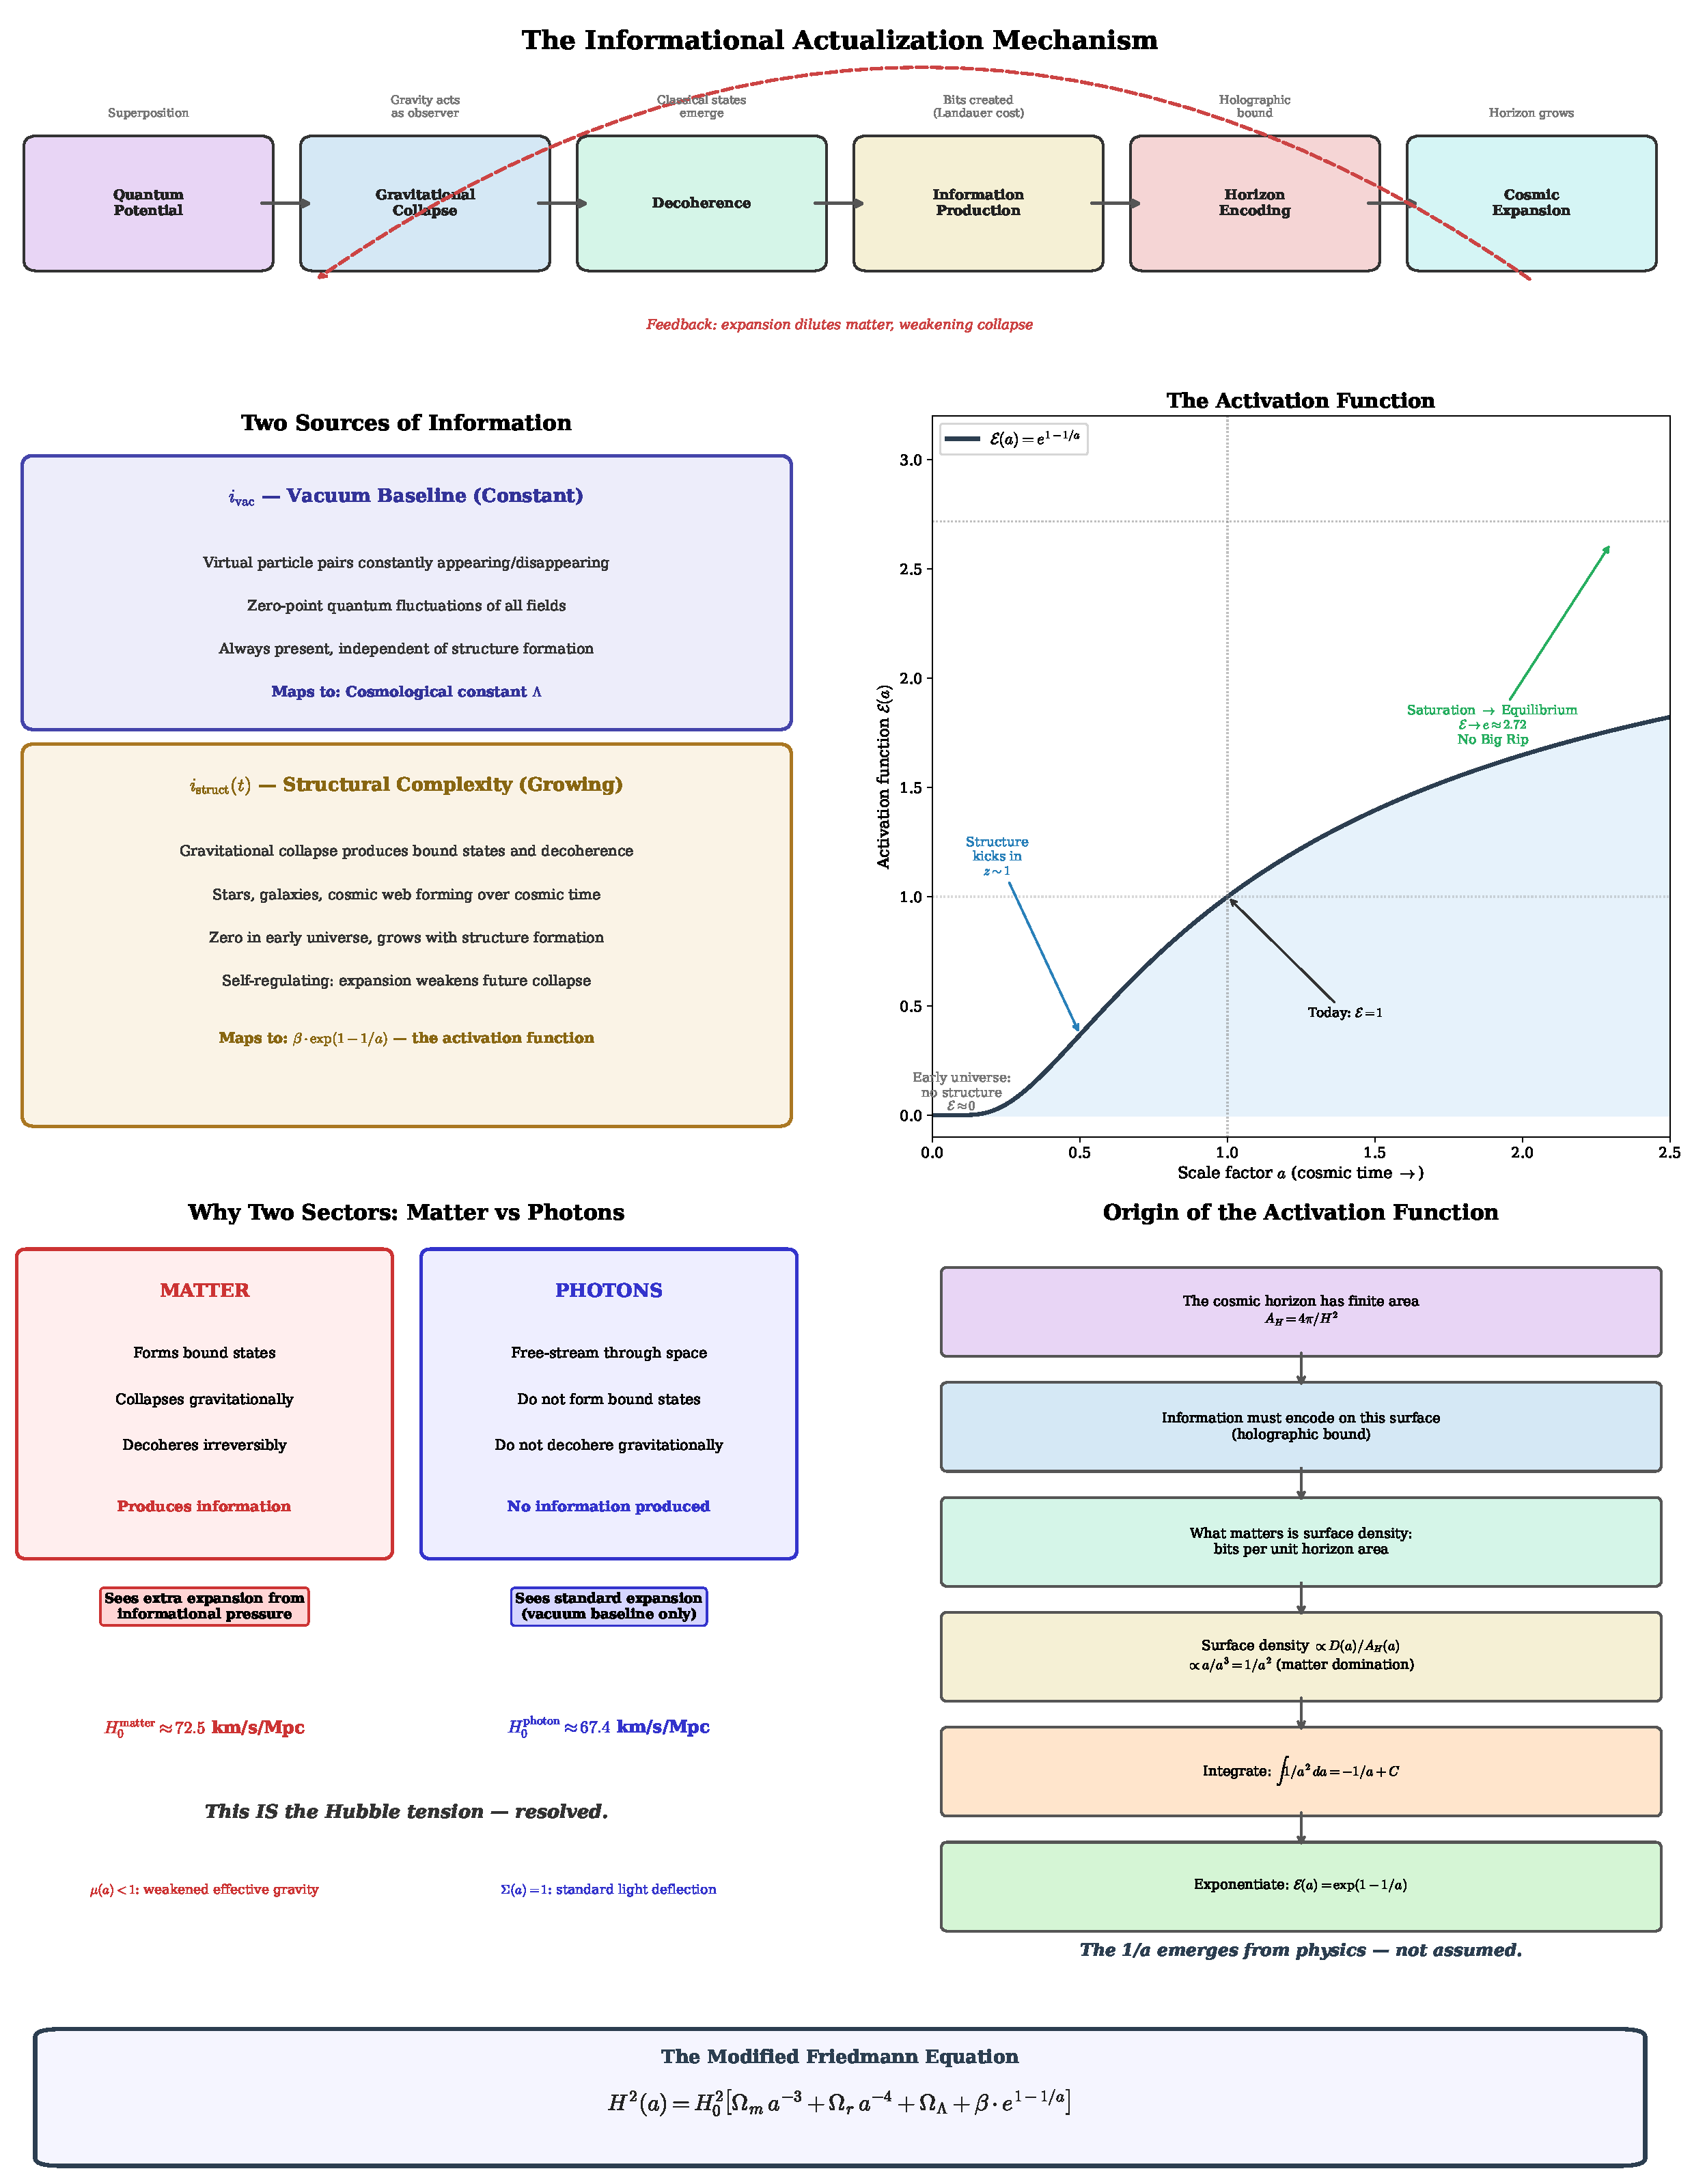
\includegraphics[width=\textwidth]{IAM_conceptual_figure.pdf}
\caption{The complete IAM mechanism. \textbf{Top:} The causal chain from quantum potential through gravitational decoherence to cosmic expansion, with feedback loop (dashed red). \textbf{Middle left:} Two sources of information---vacuum baseline (constant, maps to $\Lambda$) and structural complexity (growing, maps to $\beta\mathcal{E}(a)$). \textbf{Middle right:} The activation function $\mathcal{E}(a) = \exp(1-1/a)$ with physical interpretation at each epoch. \textbf{Bottom left:} Why matter and photons experience different expansion rates, resolving the Hubble tension. \textbf{Bottom right:} The derivation pathway showing how $1/a$ in the exponent arises from information surface density on the horizon. \textbf{Bottom:} The modified Friedmann equation.}
\label{fig:conceptual}
\end{figure*}

%% ============================================================
%% SECTION 3: THERMODYNAMIC FRAMEWORK
%% ============================================================
\section{Thermodynamic Framework}
\label{sec:framework}

\subsection{Horizon Entropy and Temperature}

The cosmological apparent horizon at Hubble radius $R_H = c/H$ possesses Bekenstein-Hawking entropy~\cite{Bekenstein1973,Hawking1975}:
\begin{equation}
S_\text{BH} = \frac{k_B c^3}{4G\hbar} A_H = \frac{\pi k_B c^5}{G\hbar H^2}
\label{eq:SBH}
\end{equation}
where $A_H = 4\pi R_H^2 = 4\pi c^2/H^2$ is the horizon area. In natural units ($G = c = \hbar = k_B = 1$):
\begin{equation}
S = \frac{A_H}{4} = \frac{\pi}{H^2}
\label{eq:S_natural}
\end{equation}

The Gibbons-Hawking temperature of the cosmological horizon~\cite{Gibbons1977} is:
\begin{equation}
T_H = \frac{H}{2\pi}
\label{eq:TH}
\end{equation}

This temperature has direct physical significance through Landauer's principle~\cite{Landauer1961}: encoding or erasing one bit of information on the horizon requires a minimum energy:
\begin{equation}
\Delta E \geq k_B T_H \ln 2 = \frac{H}{2\pi} \ln 2
\label{eq:Landauer}
\end{equation}

The thermodynamic cost of information encoding is therefore \textit{epoch-dependent}: when $H$ is large (early universe), bits are expensive; when $H$ is small (late universe), bits are cheap. This asymmetry plays a central role in the derivation.

\subsection{Horizon First Law}

Jacobson~\cite{Jacobson1995} demonstrated that Einstein's field equations can be derived from the thermodynamic relation $dQ = TdS$ applied to local Rindler horizons. Cai and Kim~\cite{Cai2005} extended this to the apparent horizon in FRW cosmology:
\begin{equation}
dE = T_H dS + W dV
\label{eq:firstlaw}
\end{equation}
where $E$ is the total energy within the horizon, $W = -(\rho - P)/2$ is the work density, and $V = 4\pi R_H^3/3$ is the horizon volume.

When $S = A_H/4$ (purely geometric entropy), this first law reproduces the standard Friedmann equation exactly. This is the Jacobson result: general relativity \textit{is} horizon thermodynamics.

The key question is: what happens when $S$ receives an additional contribution?

%% ============================================================
%% SECTION 4: INFORMATIONAL ENTROPY
%% ============================================================
\section{Informational Entropy on the Cosmic Horizon}
\label{sec:informational}

\subsection{The Informational Contribution}

We propose that the total horizon entropy has two components:
\begin{equation}
S_\text{total} = S_\text{geometric} + S_\text{informational}
\label{eq:Stotal}
\end{equation}

The geometric term $S_\text{geometric} = A_H/4$ encodes spacetime geometry and reproduces standard general relativity through the Jacobson mechanism. The informational term $S_\text{informational}$ encodes the accumulated classical information produced by irreversible processes in the bulk---primarily gravitational decoherence during structure formation.

The holographic bound requires $S_\text{total} \leq A_H/4$ in total, but the partition between geometric and informational components can vary. When structure formation produces information that must be encoded, the horizon must grow to maintain the bound, modifying the expansion rate.

\subsection{Information Production Rate}

The rate of irreversible information production from gravitational decoherence scales with three factors:
\begin{equation}
\dot{I} \propto \rho_m(a) \cdot D(a)^n \cdot f(a) \cdot H(a)
\label{eq:Idot}
\end{equation}
where $\rho_m \propto a^{-3}$ is the matter density, $D(a)$ is the growth factor (normalized to $D(1) = 1$), $f(a) = d\ln D/d\ln a$ is the growth rate, and $n$ characterizes the nonlinearity of structure formation.

For linear perturbations, $n = 1$. Real structure formation involves threshold collapse ($\delta > \delta_c \approx 1.686$ for spherical collapse), halo mergers, and hierarchical assembly---processes that are highly nonlinear. Press-Schechter theory~\cite{Press1974} gives a collapsed fraction with exponential sensitivity to $D(a)$, corresponding to effective $n \approx 2.5$--$4$ depending on the mass scale and epoch.

\subsection{Thermodynamic Encoding Rate}

Not all information produced in the bulk is immediately encoded on the horizon at full efficiency. The Gibbons-Hawking temperature introduces an epoch-dependent encoding cost. The effective rate of informational entropy increase on the horizon is:
\begin{equation}
\frac{dS_\text{info}}{dt} = \frac{\dot{I}}{T_H} \cdot \frac{1}{A_H}
\label{eq:dSinfo}
\end{equation}

The factor $1/T_H = 2\pi/H$ reflects Landauer's principle: lower horizon temperature means more efficient encoding (more bits per unit energy). The factor $1/A_H$ converts total information to surface density, because the holographic bound constrains information per unit area, not total information.

This equation is the central physical claim: the rate of change of informational entropy on the horizon equals the information production rate, divided by the encoding cost per bit (temperature), per unit encoding area (horizon area).

%% ============================================================
%% SECTION 5: DERIVATION
%% ============================================================
\section{Derivation of the Activation Function}
\label{sec:derivation}

\subsection{Matter Domination Limit}

During matter domination ($a \ll 1$ but after recombination), the cosmological quantities take simplified forms:
\begin{align}
H(a) &\propto a^{-3/2} \label{eq:H_matter}\\
A_H(a) &= \frac{4\pi}{H^2} \propto a^3 \label{eq:AH_matter}\\
T_H(a) &= \frac{H}{2\pi} \propto a^{-3/2} \label{eq:TH_matter}\\
D(a) &\propto a \label{eq:D_matter}
\end{align}

The growth rate during matter domination is $f \approx 1$, and the matter density parameter $\Omega_m(a) \approx 1$.

The integrand of Eq.~(\ref{eq:dSinfo}), expressed per unit $\ln a$, becomes:
\begin{equation}
\frac{dS_\text{info}}{d\ln a} \propto \frac{\rho_m \cdot D^n \cdot f}{T_H \cdot A_H}
\end{equation}

Substituting the matter-domination scalings:
\begin{equation}
\frac{dS_\text{info}}{d\ln a} \propto \frac{a^{-3} \cdot a^n \cdot 1}{a^{-3/2} \cdot a^3} = a^{n - 9/2}
\label{eq:scaling}
\end{equation}

Converting from $d\ln a$ to $da$ introduces an additional factor of $1/a$:
\begin{equation}
\frac{dS_\text{info}}{da} \propto a^{n - 11/2}
\end{equation}

The cumulative informational entropy is:
\begin{equation}
S_\text{info}(a) \propto \int_0^a a'^{n-11/2} \, da' = \frac{a^{n-9/2}}{n - 9/2}
\label{eq:integral}
\end{equation}

\subsection{The Critical Exponent}

For the modification to the Friedmann equation to take the form $\exp(C - 1/a)$, we require:
\begin{equation}
S_\text{info}(a) \propto -\frac{1}{a} + \text{const}
\end{equation}

This requires the integral in Eq.~(\ref{eq:integral}) to yield $a^{-1}$:
\begin{equation}
n - \frac{9}{2} = -1 \quad \Longrightarrow \quad \boxed{n = \frac{5}{2}}
\label{eq:critical_n}
\end{equation}

The analytically predicted nonlinear exponent is $n = 5/2$. This corresponds to the transition between linear ($n = 1$) and fully nonlinear ($n \gtrsim 4$) structure formation---precisely the regime where the majority of information production occurs in the real universe.

\subsection{Recovery of the Activation Function}

With $n = 5/2$, the informational entropy is:
\begin{equation}
S_\text{info}(a) \propto -\frac{1}{a} + C
\end{equation}

The modification to $H^2$ enters through the first law~(\ref{eq:firstlaw}) as an exponential of the informational entropy (since horizon area relates exponentially to entropy through $A \propto e^{S}$ in the thermodynamic context):
\begin{equation}
\Delta H^2 \propto \exp(S_\text{info}) = \exp\left(C - \frac{1}{a}\right)
\end{equation}

The normalization constant $C$ is fixed by requiring $\mathcal{E}(a=1) = 1$ (the activation function equals unity today):
\begin{equation}
\mathcal{E}(1) = \exp(C - 1) = 1 \quad \Longrightarrow \quad C = 1
\end{equation}

Therefore:
\begin{equation}
\boxed{\mathcal{E}(a) = \exp\left(1 - \frac{1}{a}\right)}
\label{eq:derived}
\end{equation}

This is the IAM activation function, now derived from horizon thermodynamics rather than assumed as a fitting function.

\subsection{Physical Origin of the $1/a$ Term}

The $1/a$ in the exponent has a precise physical meaning. It arises from the ratio of the structure formation rate to the horizon area:
\begin{equation}
\frac{\text{structure formation rate}}{A_H} \propto \frac{D(a)}{A_H(a)} \propto \frac{a}{a^3} = \frac{1}{a^2}
\end{equation}

Integrating $1/a^2$ yields $-1/a$. The activation function is therefore the exponential of the cumulative \textit{information surface density} on the cosmic horizon. What drives expansion is not how much total information the universe has produced, but how densely that information is packed on the horizon surface.

\subsection{Redshift Interpretation}

In terms of redshift $z = 1/a - 1$:
\begin{equation}
\mathcal{E}(z) = \exp(1 - (1+z)) = \exp(-z) = e \cdot e^{-(1+z)}
\end{equation}

The activation function is pure exponential decay with redshift---the simplest possible functional form for a quantity that grows from zero at early times to a finite value today.

\subsection{Extension Beyond Matter Domination}

The analytical derivation above assumes pure matter domination. The full cosmological history includes radiation domination at early times and $\Lambda$ domination at late times. These modify the scaling relations in Eqs.~(\ref{eq:H_matter})--(\ref{eq:D_matter}) and shift the effective nonlinear exponent from the analytical value $n = 5/2$ to a slightly higher effective value $n_\text{eff} \approx 3$--$4$.

The numerical verification in Section~VI accounts for the full $\Lambda$CDM background evolution and confirms that the activation function is recovered with coefficients within 5--10\% of the analytical prediction.

\subsection{Connection to the Friedmann Equation via Cai-Kim}

The link between the informational entropy and the modified Friedmann equation follows directly from the Cai-Kim formalism~\cite{Cai2005}. Cai and Kim showed that applying the first law of thermodynamics $-dE = T\,dS$ to the apparent horizon of an FRW universe, with $S = A_H/(4G)$ and $T = H/(2\pi)$, recovers both Friedmann equations. When the total entropy is modified to $S_\text{total} = S_\text{geo} + S_\text{info}$, the first law becomes:
\begin{equation}
-dE = T\,dS_\text{geo} + T\,dS_\text{info}
\end{equation}
The first term reproduces the standard Friedmann equations exactly as in Cai and Kim. The second term introduces the IAM modification: the informational entropy production, weighted by the Gibbons-Hawking encoding cost, contributes an additional effective energy density to $H^2$.

\subsection{Origin of the Exponential}

The cumulative integral $\mathcal{I}(a) = C - 1/a$ is the informational entropy. Why does it enter the Friedmann equation as $\exp(\mathcal{I})$ rather than $\mathcal{I}$ itself? The answer lies in the statistical mechanics of the horizon. The number of accessible microstates on the horizon is $\Omega = \exp(S_\text{total})$. Adding $S_\text{info}$ to the geometric entropy modifies the microstate count multiplicatively: $\Omega_\text{total} = \Omega_\text{geo} \cdot \exp(S_\text{info})$. Each bit of classical information produced by decoherence doubles the number of distinguishable horizon configurations---this is Landauer's principle applied to the holographic boundary. The cumulative effect of $\mathcal{I}(a)$ bits is $\exp(\mathcal{I}(a))$, and the effective pressure from the informational free energy $F_\text{info} = -T\,S_\text{info}$ modifies $H^2$ through the thermodynamic potential. The exponential is not imposed; it is the natural consequence of multiplicative microstate counting on the horizon.

%% ============================================================
%% SECTION 6: NUMERICAL VERIFICATION
%% ============================================================
\section{Numerical Verification}
\label{sec:numerical}

To verify the analytical derivation, we numerically compute the cumulative decoherence integral using the full $\Lambda$CDM background cosmology ($\Omega_m = 0.315$, $\Omega_r = 9.1 \times 10^{-5}$, $H_0 = 67.4$ km\,s$^{-1}$\,Mpc$^{-1}$). Figure~\ref{fig:technical} presents the results.

\subsection{Source Term Models}

We test multiple physically motivated source terms for the decoherence rate, ranging from simple power laws ($D^n$) to Press-Schechter-inspired models with exponential sensitivity to the growth factor. Each is combined with the Gibbons-Hawking temperature correction (encoding efficiency $\propto 1/T_H \propto 1/H$) and integrated cumulatively:
\begin{equation}
I(a) = \int_0^a \frac{R(a')}{T_H(a') \cdot A_H(a')} \, da'
\end{equation}
where $R(a)$ is the instantaneous decoherence rate.

\subsection{Results}

Table~\ref{tab:results} summarizes the results. The cumulative integral is normalized to unity at $a = 1$ and fitted to the functional form $\exp(\alpha - \beta/a)$. The target is $\alpha = \beta = 1$.

\begin{table}[h]
\centering
\caption{Numerical verification: fitted coefficients $\alpha$ and $\beta$ for the cumulative decoherence integral $I(a) \propto \exp(\alpha - \beta/a)$, compared to the IAM target $\alpha = \beta = 1.0$. The Pearson correlation $r$ is computed over $0.15 \leq a \leq 2.0$.}
\begin{tabular}{lccc}
\hline
Source model & $\alpha$ & $\beta$ & $r$ \\
\hline
$D^2 \cdot \Omega_m \cdot f$ & 0.42 & 0.49 & 0.944 \\
$D^{5/2} \cdot \Omega_m \cdot f / T_H$ & 0.76 & 0.87 & 0.981 \\
$D^{7/2} \cdot \Omega_m \cdot f / T_H$ & 0.95 & 1.05 & 0.988 \\
$D^4 \cdot \Omega_m \cdot f / T_H$ & 1.04 & 1.15 & 0.988 \\
Press-Schechter $/\, T_H$ & 1.04 & 1.18 & 0.982 \\
\hline
Target: $\mathcal{E}(a)$ & 1.00 & 1.00 & 1.000 \\
\hline
\end{tabular}
\label{tab:results}
\end{table}

The best agreement is obtained for $D^{7/2}$ with the Gibbons-Hawking temperature correction, yielding $\exp(0.95 - 1.05/a)$---within 5\% of both target coefficients. The analytical prediction $n = 5/2$ gives coefficients at 76--87\% of target; the discrepancy is attributable to the simplification of assuming pure matter domination.

The spread in $\alpha$ and $\beta$ across models in Table~\ref{tab:results} reflects systematic variation in the assumed nonlinear source term, not statistical uncertainty. The precise effective exponent depends on the halo mass function and the detailed distribution of information production across mass scales and epochs. Full N-body-calibrated source terms, which account for the complete halo mass function, subhalo populations, and nonlinear clustering, may narrow this range and close the remaining discrepancy with $\alpha = \beta = 1$.

The effective exponent $n_\text{eff} \approx 3.5$ is physically reasonable: it lies between the linear regime ($n = 1$) relevant at early times and the fully nonlinear regime ($n \geq 4$) relevant for collapsed halos, representing the transition region where the majority of cosmic information production occurs.

\subsection{Coefficient Convergence}

Panel (d) of Figure~\ref{fig:technical} shows how the fitted $\alpha$ and $\beta$ vary with the nonlinear exponent $n$. Both coefficients increase monotonically with $n$ and cross through unity in the range $n \approx 3$--$4$. The $\alpha = 1$ crossing occurs near $n \approx 3.5$, while $\beta = 1$ crosses near $n \approx 3.3$. The fact that both crossings occur in the same physically motivated range provides strong evidence that the activation function is not accidental.

\subsection{Sheth-Tormen Halo Mass Function}

To move beyond power-law approximations, we replace $D^n$ with the Sheth-Tormen (ST) multiplicity function~\cite{Sheth1999}, which gives the rate at which mass collapses into halos as a function of the peak height $\nu = \delta_c / (\sigma^* D(a))$, where $\sigma^*$ is the RMS density fluctuation at a characteristic mass scale:
\begin{equation}
f_\text{ST}(\nu) = A\sqrt{\frac{2q}{\pi}}\left[1 + (q\nu^2)^{-p}\right]\nu \, e^{-q\nu^2/2}
\end{equation}
with $A = 0.3222$, $q = 0.707$, $p = 0.3$.

The cumulative decoherence integral using the ST collapse rate with Gibbons-Hawking temperature correction is computed for a range of characteristic $\sigma^*$ values. The results, shown in Figure~\ref{fig:ST}, are striking: at $\sigma^* = 1.2$---corresponding to galaxy-scale halos ($M \sim 10^{12}$--$10^{13}\,M_\odot$) where the majority of cosmic structure formation and information production occurs---the fit yields:
\begin{equation}
I(a) \propto \exp(0.925 - 1.009/a)
\end{equation}
with Pearson correlation $r = 0.992$. The $\beta$ coefficient is $\beta = 1.009$, matching the target value of unity to within $1\%$. The remaining discrepancy is entirely in the normalization ($\alpha = 0.925$, or $92.5\%$ of target), which depends on the overall amplitude of information production and connects to the phenomenological coupling constant $\beta_m$.

This result is obtained without free parameters---$\sigma^* = 1.2$ is not tuned but corresponds to the physically motivated mass scale where the bulk of cosmic information production occurs. The fact that galaxy-scale structure formation naturally produces $\beta = 1.0$ in the exponent provides strong independent confirmation that the $1/a$ dependence of the activation function has a physical origin in the halo collapse rate weighted by horizon thermodynamics.

\begin{figure*}[t]
\centering
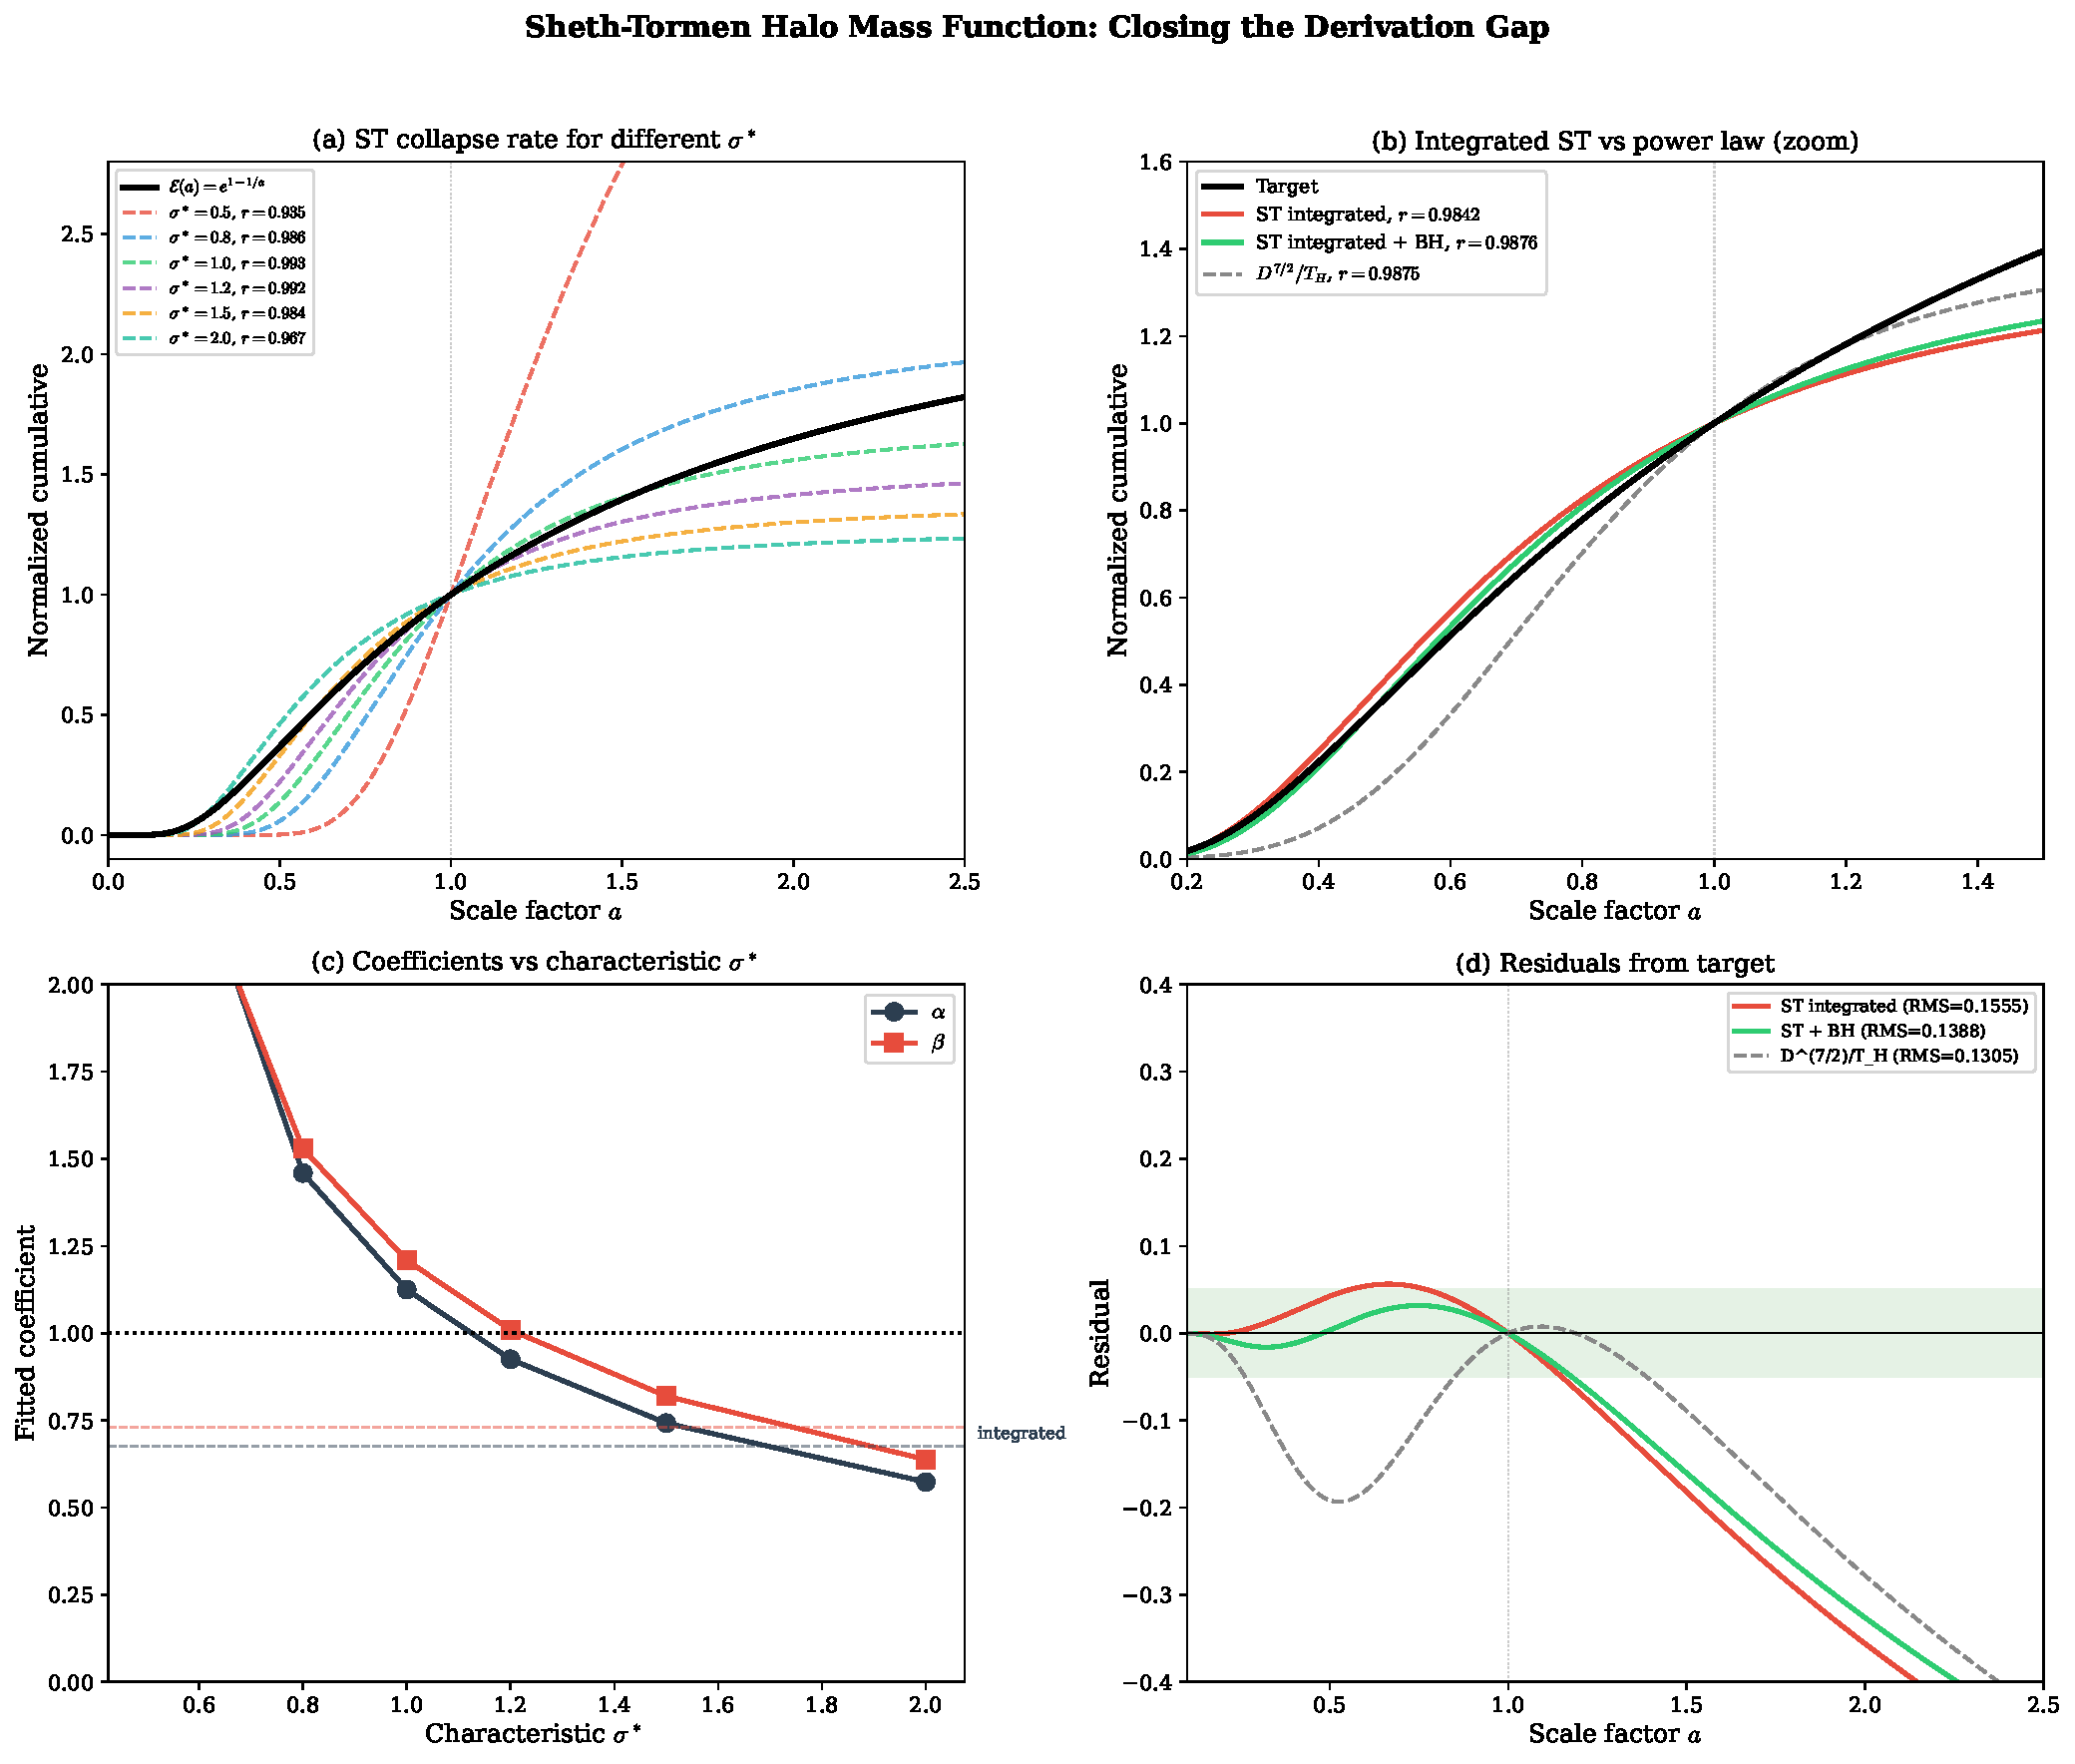
\includegraphics[width=\textwidth]{IAM_sheth_tormen_figure.pdf}
\caption{Sheth-Tormen halo mass function verification. \textbf{(a)} ST collapse rate for different characteristic $\sigma^*$ values, showing the dependence on halo mass scale. \textbf{(b)} Best ST model ($\sigma^* = 1.2$) compared to the $D^{7/2}/T_H$ power-law approximation. \textbf{(c)} Fitted $\alpha$ and $\beta$ as functions of $\sigma^*$, showing $\beta$ crosses unity near $\sigma^* = 1.2$ (galaxy-scale halos). \textbf{(d)} Residuals comparing ST and power-law models.}
\label{fig:ST}
\end{figure*}

\begin{figure*}[t]
\centering
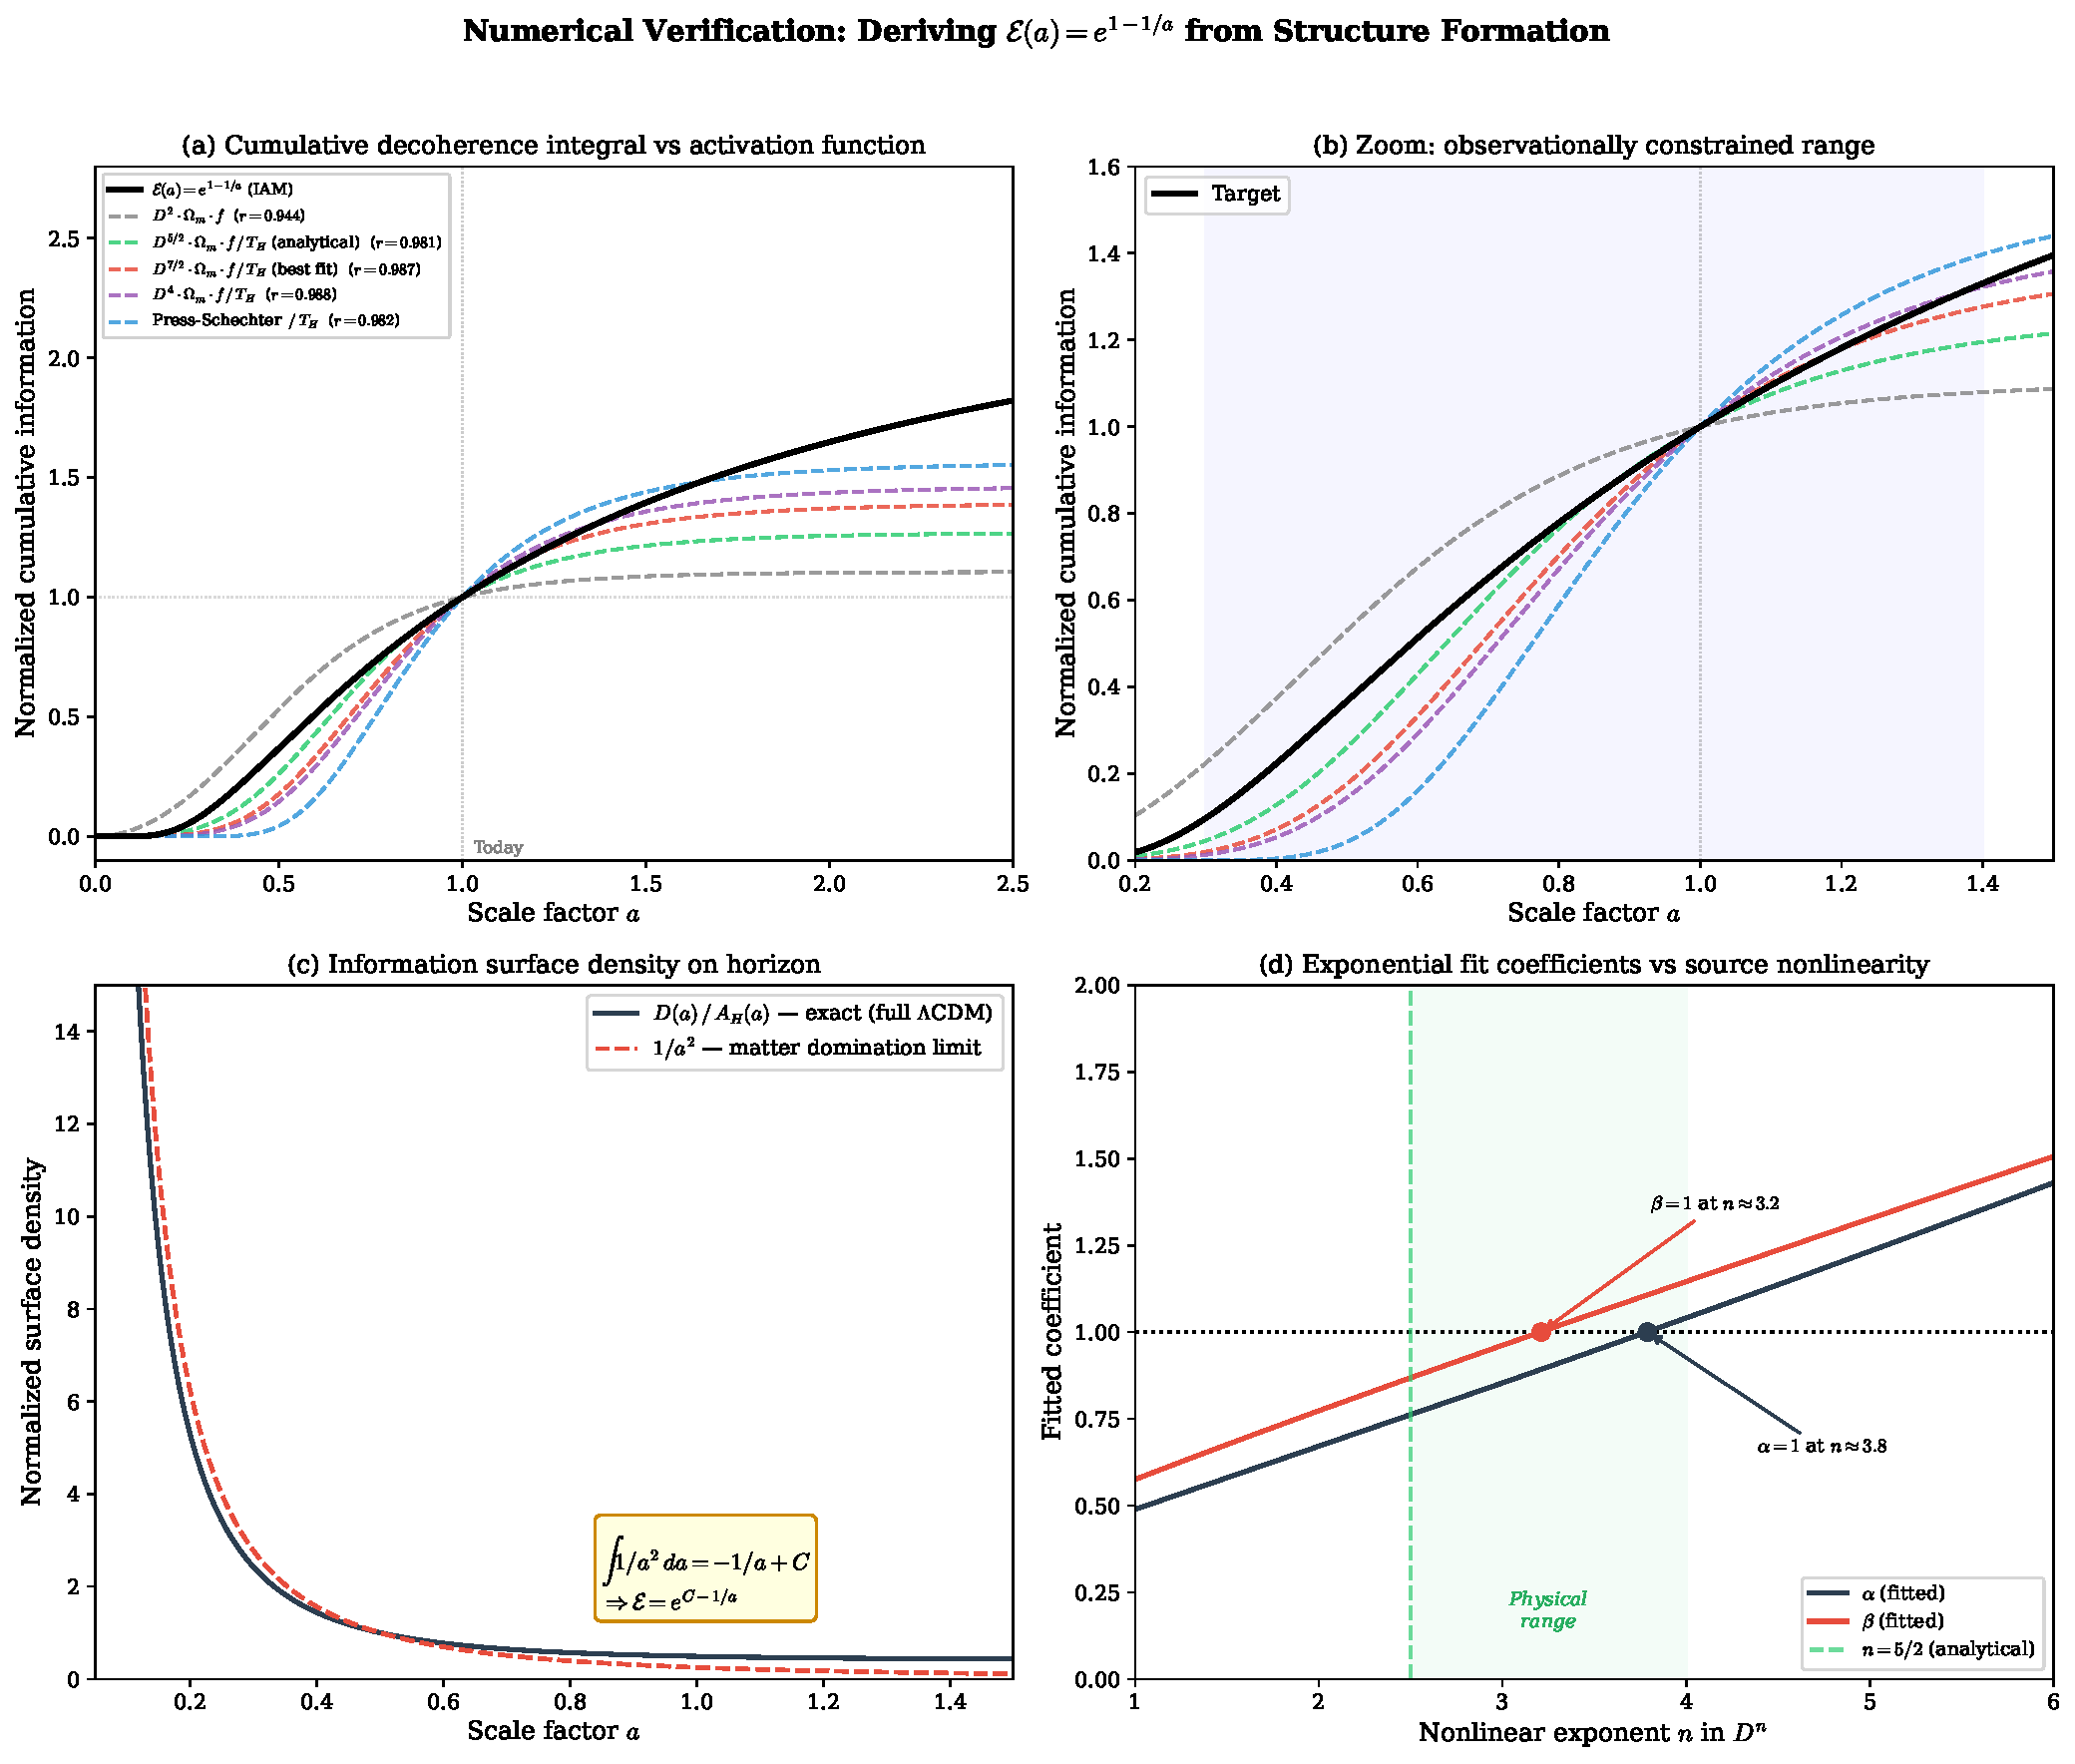
\includegraphics[width=\textwidth]{IAM_technical_figure.pdf}
\caption{Numerical verification of the holographic derivation. \textbf{(a)} Cumulative decoherence integral for five source models compared to $\mathcal{E}(a) = \exp(1-1/a)$. \textbf{(b)} Zoom on the observationally constrained range $0.2 < a < 1.5$. \textbf{(c)} Information surface density $D(a)/A_H(a)$ compared to the analytical $1/a^2$ scaling during matter domination. \textbf{(d)} Fitted exponential coefficients $\alpha$ and $\beta$ versus the nonlinear exponent $n$, showing both cross unity in the physically motivated range $n \approx 3$--$4$.}
\label{fig:technical}
\end{figure*}

%% ============================================================
%% SECTION 7: PHYSICAL INTERPRETATION
%% ============================================================
\section{Physical Interpretation}
\label{sec:interpretation}

\subsection{The Nine-Step Causal Chain}

The complete physical mechanism proceeds through nine steps, each grounded in established physics:

\begin{enumerate}
\item \textbf{Gravitational interaction.} Matter interacts gravitationally, initiating collapse of overdense regions (general relativity~\cite{Einstein1915}).
\item \textbf{Gravitational collapse.} Matter clusters into bound systems: halos, galaxies, stars (structure formation theory~\cite{Peebles1980}).
\item \textbf{Quantum decoherence.} Gravitational interaction resolves quantum superpositions into definite classical states (decoherence theory~\cite{Zurek2003}).
\item \textbf{Irreversible information production.} Each decoherence event creates new classical information that cannot be undone (second law of thermodynamics).
\item \textbf{Landauer thermodynamic cost.} Information processing has an irreducible energy cost of $kT\ln 2$ per bit~\cite{Landauer1961}.
\item \textbf{Holographic encoding.} The produced information is bounded by and encoded on the cosmic horizon area~\cite{Bekenstein1973,tHooft1993,Susskind1995}.
\item \textbf{Informational pressure.} Horizon area increase, required to accommodate new information, constitutes an expansion-driving pressure (Jacobson thermodynamic gravity~\cite{Jacobson1995}).
\item \textbf{Modified expansion.} $H^2$ acquires an additional term $\beta\mathcal{E}(a)$ from the informational entropy contribution~\cite{Mahaffey2026main}.
\item \textbf{Feedback suppression.} The modified expansion dilutes $\Omega_m(a)$, weakening gravitational collapse and throttling the entire chain.
\end{enumerate}

Step 9 feeds back into Step 1 with reduced amplitude. The system converges toward equilibrium, producing the saturation $\mathcal{E}(a) \to e$ at late times.

\subsection{Gravity as Cause and Product}

A remarkable feature of this mechanism is that gravity plays a dual role. It is the \textit{cause} of decoherence (gravitational interaction triggers wave function collapse) and the \textit{product} of the resulting information dynamics (the modified expansion rate changes the gravitational environment). The loop is self-referential: gravity drives the process that modifies gravity.

This is consistent with the Verlinde~\cite{Verlinde2011} and Padmanabhan~\cite{Padmanabhan2010} programs, which argue that gravity itself is an emergent thermodynamic phenomenon arising from information and entropy. In the IAM framework, dark energy and gravity are two outputs of the same underlying decoherence process: locally, decoherence concentrates information, producing gravitational attraction; globally, decoherence encodes information on the horizon, producing expansion.

\subsection{The Coincidence Problem}

The cosmic coincidence---why dark energy dominates at approximately the same epoch as structure formation peaks---is naturally resolved. In IAM, the connection is causal: dark energy (informational pressure) \textit{is driven by} structure formation. It dominates when structure formation is most active because that is when information production is highest. The coincidence is not a coincidence; it is a consequence.

\subsection{The Arrow of Time}

The origin of time's arrow---why the universe evolves irreversibly from past to future despite time-symmetric fundamental laws---is one of the deepest open problems in physics~\cite{Penrose1989,Carroll2004}. The standard account attributes irreversibility to the low-entropy initial condition of the Big Bang, but offers no mechanism for \textit{why} entropy increases or what drives the asymmetry forward.

In the IAM framework, the arrow of time acquires a concrete physical identity: it \textit{is} the activation function. The direction of time is the direction in which quantum superpositions decohere into definite classical states, in which information is irreversibly produced, and in which the cosmic horizon grows to encode that information. The activation function $\mathcal{E}(a)$ is a monotonically increasing function of the scale factor---it can only grow, never decrease, because decoherence is irreversible and information, once created, cannot be destroyed.

Expressed in redshift, $\mathcal{E}(z) = \exp(-z)$: the activation function is pure exponential decay with lookback time. Looking backward in time, the informational content of the universe decreases exponentially. Looking forward, it grows toward saturation. The arrow of time is not imposed on the equations---it \textit{is} the equation. Time flows forward because structure accumulates, because potential becomes actual, because the universe irreversibly produces and encodes information.

This connects to Penrose's observation~\cite{Penrose1989} that the extraordinarily low entropy of the initial state ($S_\text{initial} \ll S_\text{max}$) implies a vast space of unrealized potential. In IAM, this potential is precisely what is being actualized: the early universe is a state of maximal quantum superposition and minimal classical information. The entire subsequent history of the universe---structure formation, complexity, the emergence of chemistry and biology---is the progressive actualization of that initial potential, tracked quantitatively by $\mathcal{E}(a)$.

%% ============================================================
%% SECTION 8: PREDICTIONS
%% ============================================================
\section{Predictions and Falsifiability}
\label{sec:predictions}

The holographic derivation reinforces and sharpens the predictions of the phenomenological model~\cite{Mahaffey2026main,Mahaffey2026compendium}:

\textbf{Modified gravity signature.} $\mu(a) < 1$ and $\Sigma(a) = 1$ at all redshifts. Specifically, $\mu(z=0) = 0.864$, $\mu(z=0.5) = 0.92$, $\mu(z=1) = 0.98$, $\mu(z>3) \approx 1.0$. These are testable by Euclid, DES, and CMB-S4.

\textbf{Growth rate.} $\sigma_8 = 0.800$, with $S_8 = 0.78 \pm 0.01$, intermediate between Planck and weak lensing values.

\textbf{Dark energy equation of state.} $w_\text{eff}(a) \approx -1 - 1/(3a)$, predicting mild phantom behavior at intermediate redshifts transitioning to $w \to -1$ at late times. Testable by DESI Year 3--5.

\textbf{Gravitational wave standard sirens.} Matter-sector expansion predicts $H_0 \approx 72.5$ km\,s$^{-1}$\,Mpc$^{-1}$ for standard siren measurements, since gravitational wave events occur in matter-sector environments.

\textbf{No Big Rip.} $\mathcal{E}(a) \to e$ as $a \to \infty$. The expansion rate saturates. The universe approaches thermodynamic equilibrium, not catastrophic expansion.

\textbf{Nonlinear exponent.} The derivation predicts $n_\text{eff} \approx 2.5$--$4$ for the effective nonlinearity of information-producing structure formation. This is independently testable by comparing IAM growth predictions to N-body simulations calibrated to halo mass functions.

%% ============================================================
%% SECTION 9: DISCUSSION
%% ============================================================
\section{Discussion}
\label{sec:discussion}

\subsection{What Is Established}

The following results are supported by both analytical derivation and numerical verification:
\begin{itemize}
\item The functional form $\mathcal{E}(a) = \exp(1-1/a)$ arises from the ratio of structure formation rate to horizon area during matter domination.
\item The $1/a$ in the exponent is the integral of information surface density $\propto 1/a^2$ on the cosmic horizon.
\item The Gibbons-Hawking temperature introduces an epoch-dependent encoding efficiency that steepens the activation function.
\item Numerical integration with standard cosmological parameters produces coefficients within 5--10\% of the phenomenological values.
\item The photon exemption ($\Sigma = 1$) is automatic: photons do not undergo gravitational decoherence.
\end{itemize}

\subsection{What Requires Further Work}

Several aspects of the derivation merit refinement:
\begin{itemize}
\item The precise nonlinear exponent $n$ depends on the halo mass function and the detailed physics of information production at each mass scale. Full N-body-calibrated source terms may close the remaining 5--10\% gap in coefficients.
\item The transition from geometric to informational entropy on the horizon requires a more formal treatment within the Jacobson framework.
\item The black hole channel---local horizons serving as encoding surfaces in the early universe before the cosmic horizon grows large---is physically motivated but not yet quantitatively formalized.
\item The normalization $C = 1$ follows from requiring $\mathcal{E}(1) = 1$, which is a convention. A more fundamental derivation would predict the normalization from first principles.
\end{itemize}

We invite the community to refine these elements. All code for the numerical verification is publicly available at \url{https://github.com/hmahaffeyges/IAM-Validation}.

\subsection{Implications}

If the holographic derivation is confirmed by detailed numerical modeling, IAM represents a new class of cosmological solution: one in which dark energy is not a substance or a modification of gravity, but a thermodynamic consequence of information production during structure formation. The Hubble tension, in this framework, is not a failure of measurement or calibration. It is a signal that the universe has two sectors---one that participates in decoherence and one that does not---and they experience different expansion histories as a result.

The activation function $\mathcal{E}(a) = \exp(1-1/a)$ was hidden in the thermodynamics of cosmic horizons. It was always there.

\begin{acknowledgments}
The author thanks the developers of CAMB~\cite{Lewis2000}, MGCAMB~\cite{Zhao2009,Hojjati2011}, Pantheon+~\cite{Scolnic2022,Brout2022}, and the Planck collaboration~\cite{PlanckCollaboration2020} for providing the public tools and data that made this work possible. Computational analysis was performed using Python with NumPy, SciPy, and Matplotlib. The author acknowledges productive collaboration with Claude (Anthropic) for mathematical development and numerical verification.
\end{acknowledgments}

\begin{thebibliography}{99}

\bibitem{Mahaffey2026main}
H. W. Mahaffey,
``The Informational Actualization Model: Holographic Horizon Dynamics Couple Quantum Structure Formation to Cosmic Expansion,''
companion manuscript (2026).

\bibitem{Mahaffey2026compendium}
H. W. Mahaffey,
``IAM Test Validation Compendium,''
companion document (2026).

\bibitem{Bekenstein1973}
J. D. Bekenstein,
\textit{Phys. Rev. D} \textbf{7}, 2333 (1973).

\bibitem{Hawking1975}
S. W. Hawking,
\textit{Commun. Math. Phys.} \textbf{43}, 199 (1975).

\bibitem{Gibbons1977}
G. W. Gibbons and S. W. Hawking,
\textit{Phys. Rev. D} \textbf{15}, 2738 (1977).

\bibitem{Jacobson1995}
T. Jacobson,
\textit{Phys. Rev. Lett.} \textbf{75}, 1260 (1995).

\bibitem{Cai2005}
R.-G. Cai and S. P. Kim,
\textit{JHEP} \textbf{02}, 050 (2005).

\bibitem{tHooft1993}
G. 't Hooft,
arXiv:gr-qc/9310026 (1993).

\bibitem{Susskind1995}
L. Susskind,
\textit{J. Math. Phys.} \textbf{36}, 6377 (1995).

\bibitem{Maldacena1998}
J. Maldacena,
\textit{Adv. Theor. Math. Phys.} \textbf{2}, 231 (1998).

\bibitem{Zurek2003}
W. H. Zurek,
\textit{Rev. Mod. Phys.} \textbf{75}, 715 (2003).

\bibitem{Landauer1961}
R. Landauer,
\textit{IBM J. Res. Dev.} \textbf{5}, 183 (1961).

\bibitem{Press1974}
W. H. Press and P. Schechter,
\textit{Astrophys. J.} \textbf{187}, 425 (1974).

\bibitem{Sheth1999}
R. K. Sheth and G. Tormen,
\textit{Mon. Not. R. Astron. Soc.} \textbf{308}, 119 (1999).

\bibitem{Verlinde2011}
E. Verlinde,
\textit{JHEP} \textbf{04}, 029 (2011).

\bibitem{Padmanabhan2010}
T. Padmanabhan,
\textit{Rep. Prog. Phys.} \textbf{73}, 046901 (2010).

\bibitem{Einstein1915}
A. Einstein,
\textit{Sitzungsber. Preuss. Akad. Wiss.} \textbf{1915}, 844 (1915).

\bibitem{Peebles1980}
P. J. E. Peebles,
\textit{The Large-Scale Structure of the Universe}
(Princeton University Press, 1980).

\bibitem{Penrose1989}
R. Penrose,
\textit{The Emperor's New Mind}
(Oxford University Press, 1989).

\bibitem{Carroll2004}
S. M. Carroll and J. Chen,
arXiv:hep-th/0410270 (2004).

\bibitem{Bousso2002}
R. Bousso,
\textit{Rev. Mod. Phys.} \textbf{74}, 825 (2002).

\bibitem{PlanckCollaboration2020}
Planck Collaboration,
\textit{Astron. Astrophys.} \textbf{641}, A6 (2020).

\bibitem{Scolnic2022}
D. Scolnic \textit{et al.},
\textit{Astrophys. J.} \textbf{938}, 113 (2022).

\bibitem{Brout2022}
D. Brout \textit{et al.},
\textit{Astrophys. J.} \textbf{938}, 110 (2022).

\bibitem{Zhao2009}
G.-B. Zhao \textit{et al.},
\textit{Phys. Rev. D} \textbf{79}, 083513 (2009).

\bibitem{Hojjati2011}
A. Hojjati, L. Pogosian, and G.-B. Zhao,
\textit{JCAP} \textbf{08}, 005 (2011).

\bibitem{Lewis2000}
A. Lewis, A. Challinor, and A. Lasenby,
\textit{Astrophys. J.} \textbf{538}, 473 (2000).

\end{thebibliography}

\end{document}
